\documentclass{article}
\usepackage[utf8]{inputenc}

\title{Røde Kors mast manual}
\author{Øystein Smith}
\date{September 2018}

\usepackage{natbib}
\usepackage{graphicx}
\usepackage{subcaption}
\captionsetup{compatibility=false}
\usepackage{cleveref}
\begin{document}

\maketitle

\section{Introduction}
This short manual is for the mast known as CMC TYPE 406/654/1 also known as AB-952. Originaly made for the AN/GRC-103(V) radio system. In \cref{fig:labels} the labels attached to the mast launcher (base) is shown.

\begin{figure}[h!]
	\centering
	\begin{subfigure}{.5\textwidth}
		\centering
		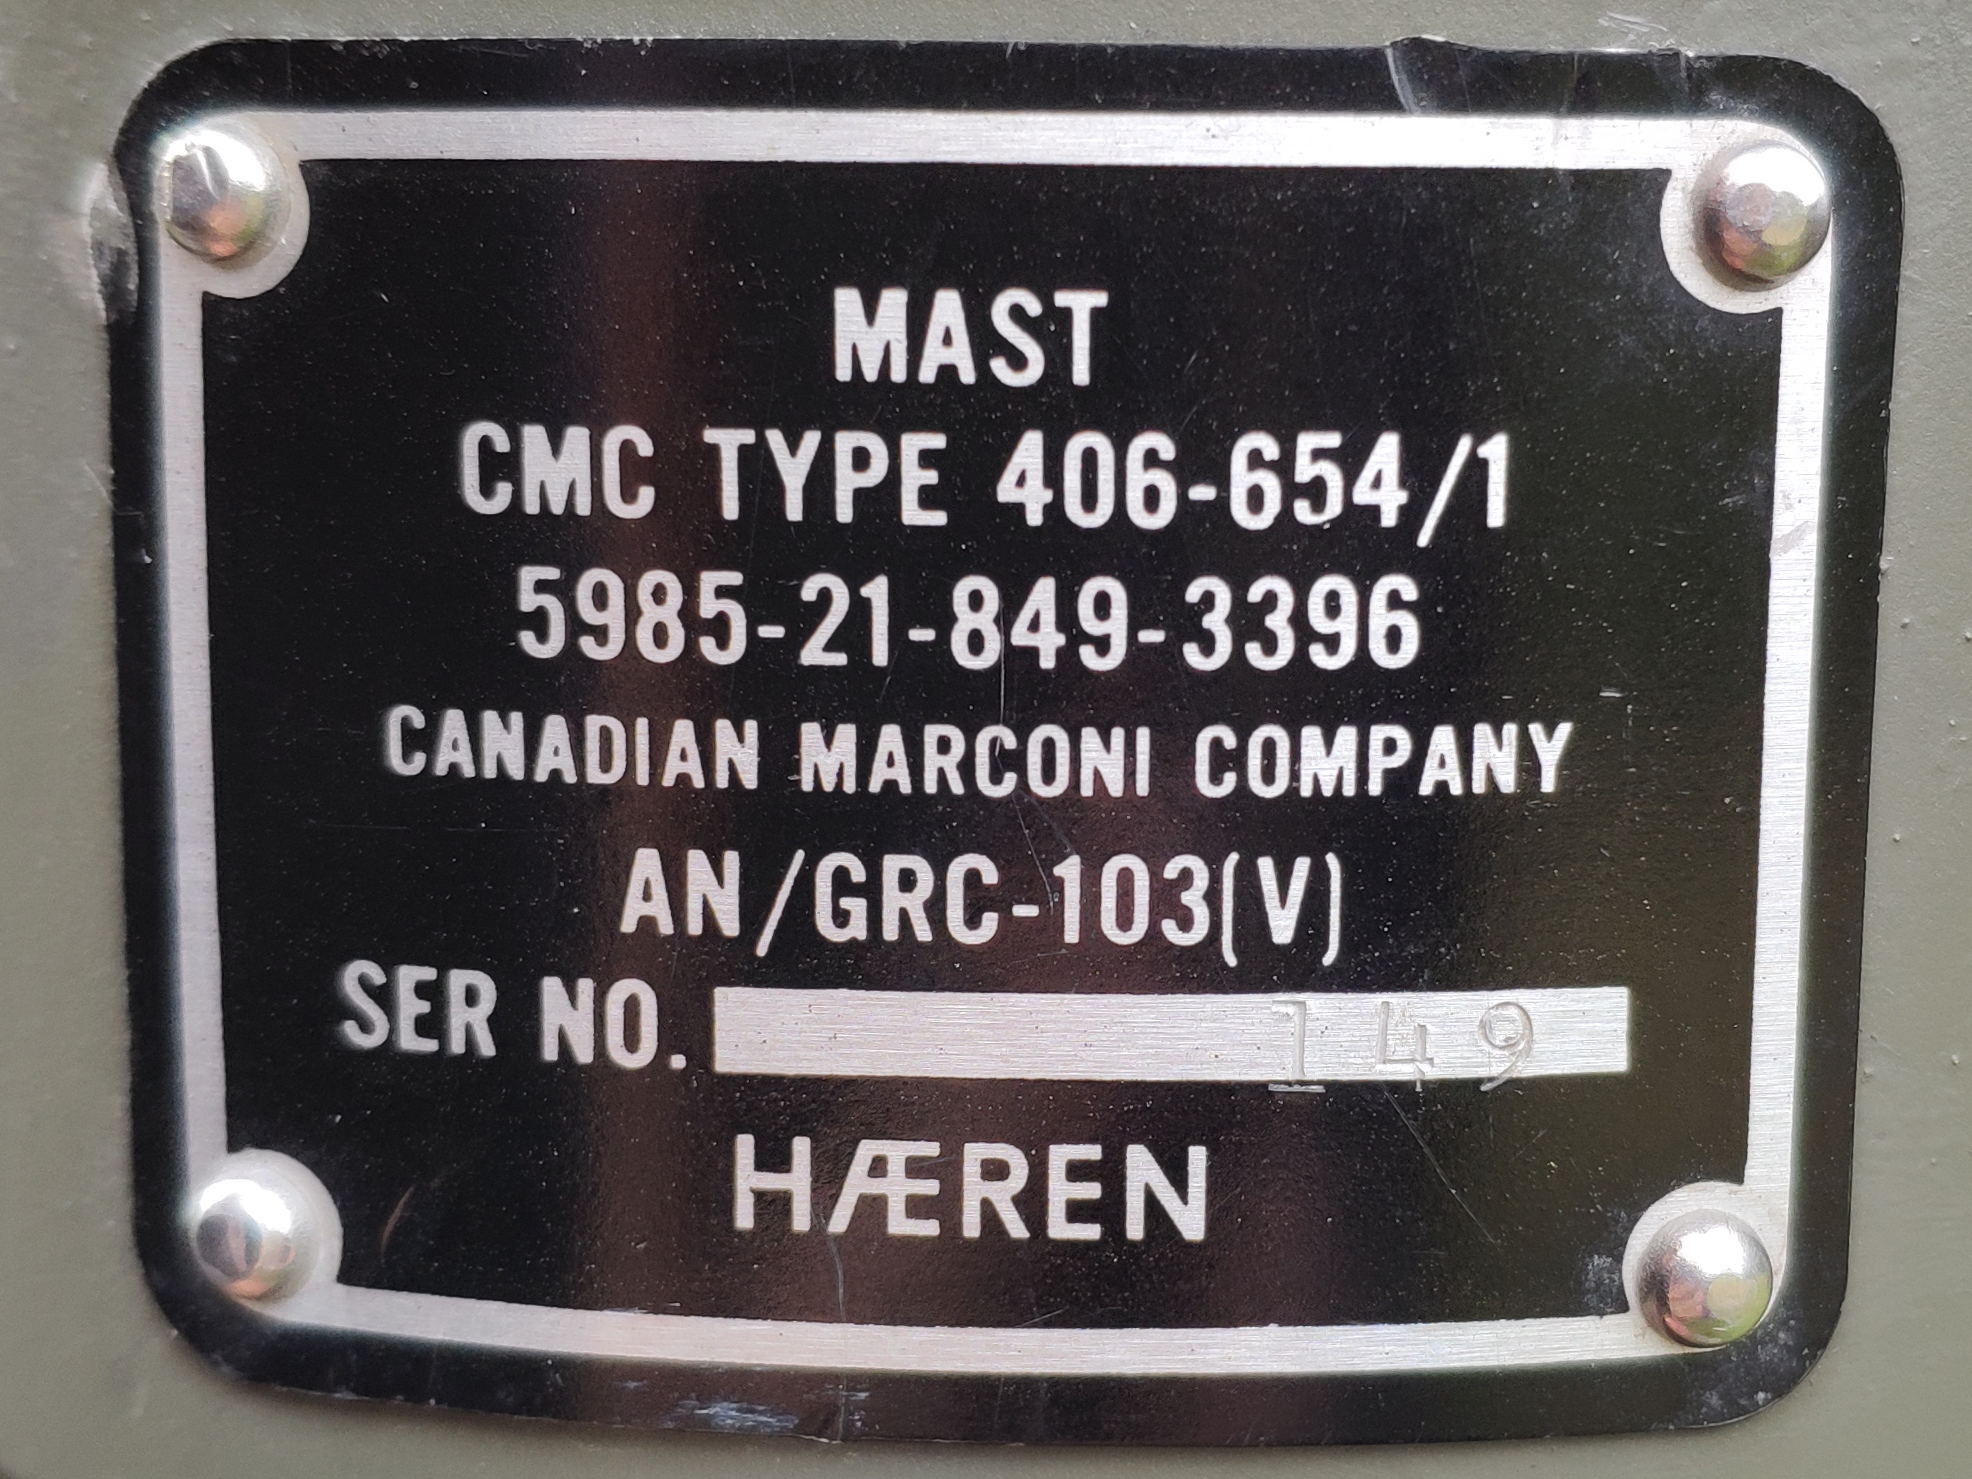
\includegraphics[width=\linewidth]{img/Label1.jpg}
		\caption{Hæren label}
		\label{fig:label1}
	\end{subfigure}%
    ~
	\begin{subfigure}{.5\textwidth}
		\centering
		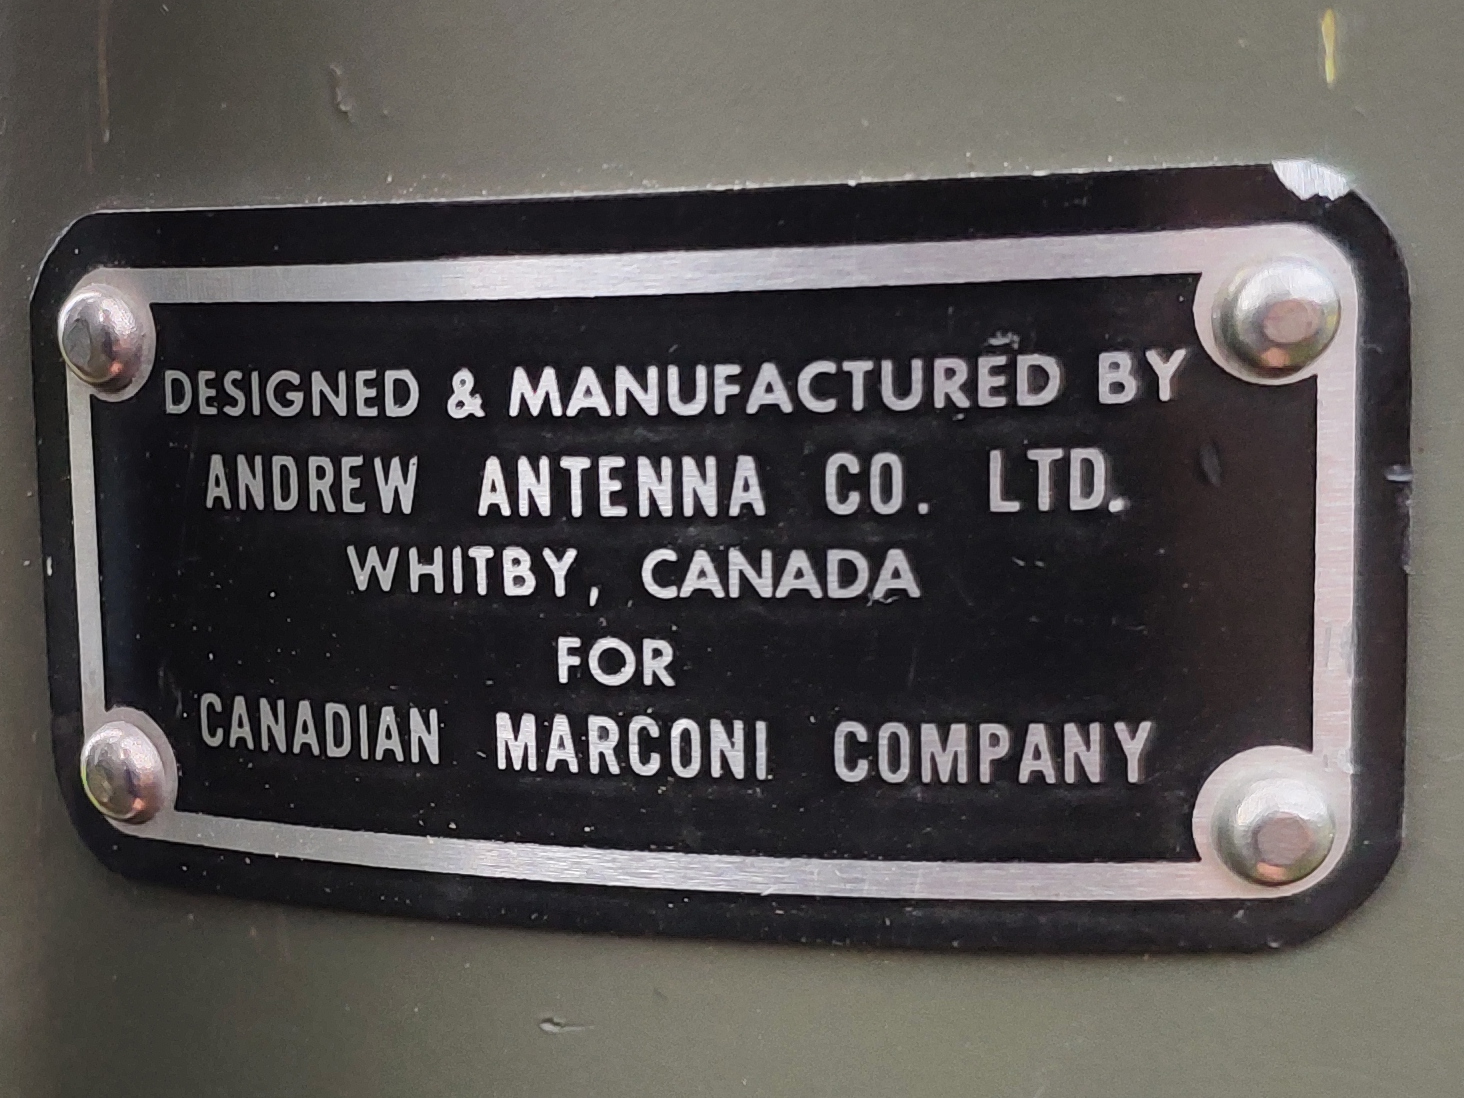
\includegraphics[width=\linewidth]{img/Label2.jpg}
		\caption{Manufacturer label}
		\label{fig:label2}
	\end{subfigure}
	\caption{Labels on the mast}
	\label{fig:labels}
\end{figure}

\subsection{Components}
The mast consists of
\begin{itemize}
\item Launcher
\item Seven mast sections
\item Top section
\item Three short guys (marked with red)
\item Three long guys
\item Three nails
\item Three long plugs
\item Three short plugs
\item Hammer
\end{itemize}

\section{Preparing}
First find a suitable location to erect the mast. The location has to havea flat area for the launcher with some soil to attach the launcher to the ground with plugs. A couple of meters clearing around the launcher, and clearing for three guy wires spaced 120 degrees about eight meters out from the launcher.

Then position the launcher in the middle of the suitable location and remove the mast sections from the launcher.

Isert the three long nails (about 20cm long) in the three holes in the bottom of the launcher marked with yellow to attach the launcher to the ground and prevent it from sliding sideways.

Then take out the three short guys, marked with red. And attach (either end) to the rings marked with red on the launcher. Stretch the guys out to about 4-8 meters from the launcher spaced 120 degrees from eachother, preferably one straight into the wind direction.

Then attach the top section to the mast section that is in the launcher.
This is a good time to attach the antenna or other things that should be in the top of the mast. There is a good idea to attach a ring (or several)  with a rope at least twice the length of the mast so you can hoist up stuff in the mast. For example one end of a wire dipole antenna.

Then attach the three long guys to the (rings on the) top section of the mast.

\section{Guying}

\section{Extending the launcher}

\section{Jacking up the mast}

\section{Lowering the mast}

\section{Stowing the mast}

\end{document}

